\documentclass{article}
\usepackage{graphicx}
\usepackage[margin=1.5cm]{geometry}
\usepackage{amsmath}

\begin{document}
\twocolumn

\title{Wednesday warm-up: Forces IV}
\author{Prof. Jordan C. Hanson}

\maketitle

\section{Memory Bank}

\begin{itemize}
\item Spring force: $\vec{s} = -k \Delta \vec{x}$, where $k$ is the spring constant and $\Delta\vec{x}$ is the displacement.
\item Young's Modulus, $Y$, has units of N m$^{-2}$, and it relates the change in length $\Delta L$ of a system of original length $L_0$ and cross-sectional area $A$ subject to a force $F$:
\begin{equation}
\frac{\Delta L}{L_0} = \frac{1}{Y} \frac{F}{A}
\end{equation}
\item Shear Modulus, $S$, has units of N m$^{-2}$, and it relates the sideways change in length $\Delta x$ of a system of length $L_0$ and cross-sectional area $A$ subject to a force $F$:
\begin{equation}
\frac{\Delta x}{L_0} = \frac{1}{S} \frac{F}{A}
\end{equation}
\end{itemize}

\section{Springs and Restoring Forces}

\begin{enumerate}
\item Calculate the change in length of the upper leg bone (the femur) when a 70.0 kg man supports 62.0 kg of his mass on it, assuming the bone to be equivalent to a uniform rod that is 40.0 cm long and 2.00 cm in radius. Young's Modulus for bone is $9 \times 10^9$ N m$^{-2}$. \\ \vspace{3cm}
\item Find the mass of the picture hanging from a steel nail, given that the nail bends only 1.80 microns ($10^{-6}$ m).  The shear modulus is $80 \times 10^9$ N m$^{-2}$. \\ \vspace{3cm}
\item Suppose three springs with equal $k$ constants are connected \textit{in series} (back to back).  If the springs have original length $L_0$, what is the total length if a mass $m$ is hung from them?
\end{enumerate}

\begin{figure}[hb]
\centering
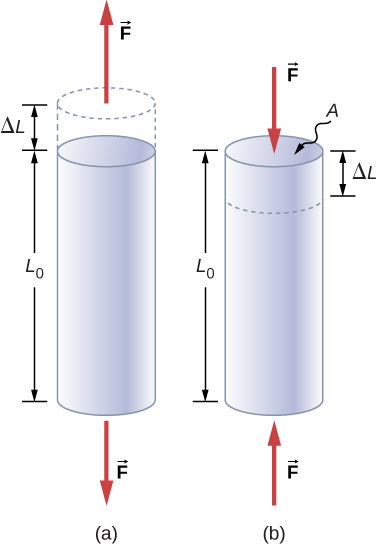
\includegraphics[width=0.2\textwidth]{figures/strain.jpeg}
\caption{\label{fig:2} Stress equals Y times strain.}
\end{figure}

\begin{figure}[hb]
\centering
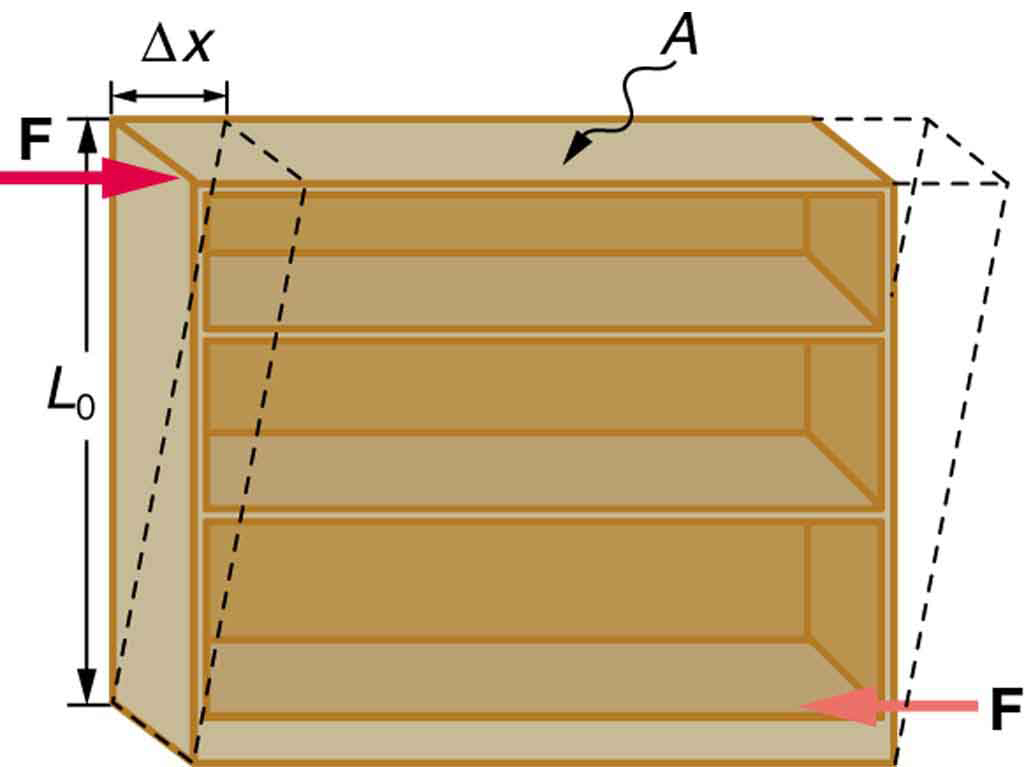
\includegraphics[width=0.25\textwidth]{figures/shelf.jpeg}
\caption{\label{fig:3} Stress equals S times shear.}
\end{figure}

\begin{figure}[hb]
\centering
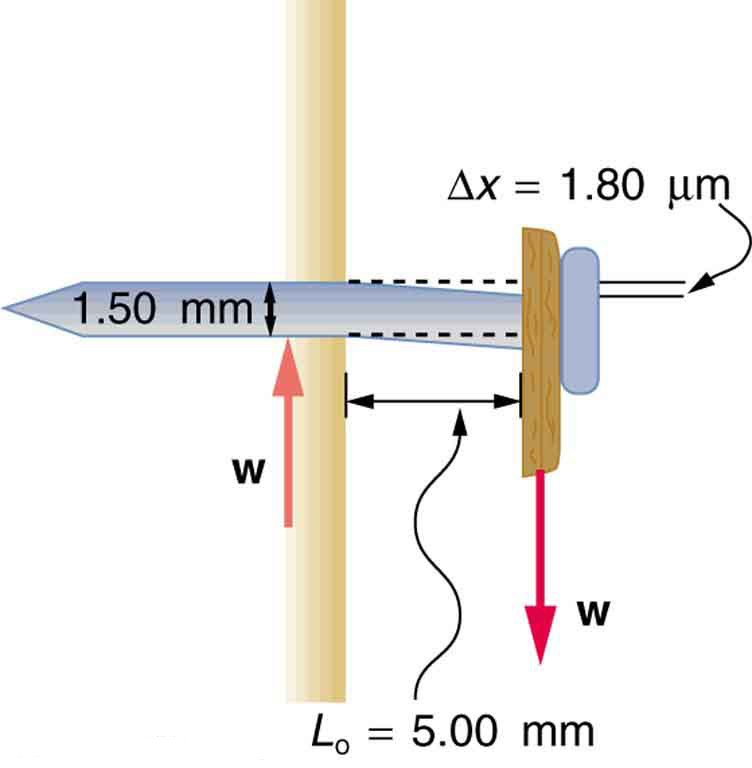
\includegraphics[width=0.25\textwidth]{figures/nail.jpeg}
\caption{\label{fig:3} Stress equals S times shear.}
\end{figure}


\end{document}
